
\label{Monopix1}
\begin{titlepage}

\section{TJ-Monopix1}

TJ 180 nm CMOSS process was firstly used for Alice inner tracker system: ALPIDE
(primo ad avere FE sul pixel e sparsiefied zero suppression readout).

TJ monopix ha un colum drain readout proven by the ATLAS FEI3 front end chip (
I. Peric et al., The FEI3 readout chip for the ATLAS pixel detector,
Nucl. Instrum. Meth. A 565 (2006) 178, ed. by J. Grosse-Knetter, H. Krueger, and N. Wermes
(cit. on pp. 42, 50, 60))\\

Epitaxial layer thickness: più grande è e più carica viene depositata da una MIP,
però devi fare attenzione alla forma della zona svuotata perchè può portare ad un
aumento della charge sharing tra pixel vicini.
Se il diodo è molto piccolo rischi che l'efficienza di collection è diminutia perchè
l'intensità del campo elettrico è più bassa intorno al diodo, e hai più charge sharing.

50x50 um2 e l'elettrodo è 3 um

INput coupling: differenza tra AC (flavor HV) e DC. 4 flavors\\



\subsection{FE}
R resistenza di reset deve essere abbastanza grande in modo da far si che il
ritorno allo zero è abbastanza lento (non devi "interferire" con la tot slope
e non devi più corto del tempo del preamplificatore, sennò hai perdita di segnale).\\
Baseline reset: all'input solitamente hai un PMOSS o un diodo;  


\begin{figure}
    \centering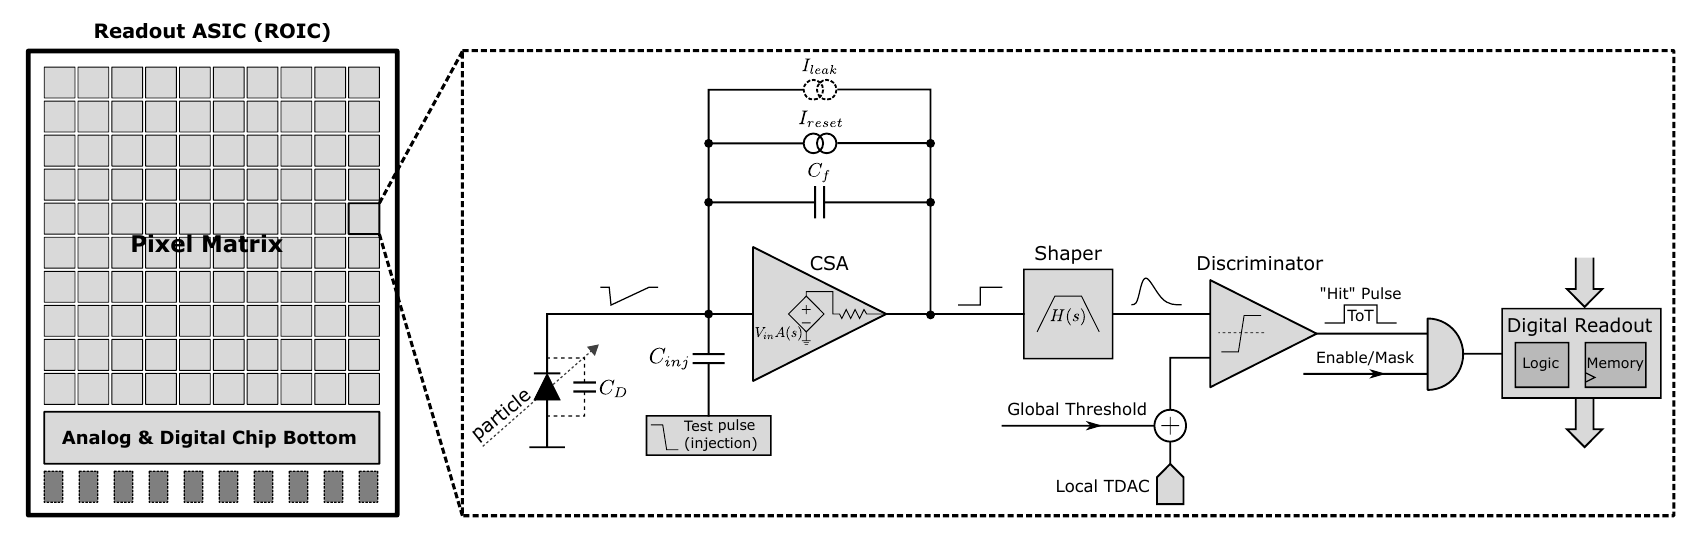
\includegraphics[width=15cm]{figures/readout_scheme.png}
    \caption{Readout FE scheme}
    \label{fig:readout_scheme}
    \end{figure}
Voltage amplifier: perchè? ripeti un attimo il vantaggio. \\
Source follower per disaccoppiare shaper e LF feedback.\\

\subsection{Readout architecture}
viene da lf monopix\\
\end{titlepage}
